\documentclass[a4paper,12pt]{extarticle}

\usepackage[utf8]{inputenc}
\usepackage[T1]{fontenc} %Not needed by LuaLaTeX or XeLaTeX
\usepackage[french]{babel}
\usepackage[autolanguage]{numprint} % for the \nombre command
\usepackage{fancyhdr}
\usepackage{vmargin}
%\usepackage{hyperref}
\usepackage{graphicx}
\usepackage{hyperref}
\usepackage{caption}
\usepackage{hyphenat}
\hyphenation{mate-mática recu-perar}
\usepackage{url}
\usepackage{amsmath}
\usepackage{mathtools}
\usepackage{hyperref}
\usepackage{color}
\usepackage{enumitem,amssymb}
\newlist{todolist}{itemize}{2}
\setlist[todolist]{label=$\square$}
\usepackage{pifont}
\newcommand{\cmark}{\ding{51}}%
\newcommand{\xmark}{\ding{55}}%
\newcommand{\done}{\rlap{$\square$}{\raisebox{2pt}{\large\hspace{1pt}\cmark}}}
\newcommand{\fail}{\rlap{$\square$}{\large\hspace{1pt}\xmark}}

\setmarginsrb{2cm}{1cm}{2cm}{1cm}{1cm}{1cm}{1cm}{1cm}

\title{Présentation : \\ Contrôle de la trajectoire}
\author{Léon J-H}

\pagestyle{fancy}
\fancyhf{}
\rhead{Léon J-H}
\lhead{Contrôle de la trajectoire}
\cfoot{\thepage}

\begin{document}

\begin{titlepage}
    \centering
    \vspace*{0.5 cm}
	{ \Huge{\bfseries{Présentation : \\ Contrôle de la trajectoire}}}\\
	\vspace*{0.5 cm}
	\rule{\linewidth}{0.2 mm} \\[1 cm]

\tableofcontents
\pagebreak


\end{titlepage}

\section{Introduction}
\subsection{Contexte : Formule ÉTS - voiture autonome}

Dans le cadre de la Formule ÉTS, il y a un département driverless, je suis en charge de faire \textbf{le contrôle de la trajectoire}, mais aussi de faire l'algorithme de planification de la trajectoire.

\begin{figure}[h]
    \centering
    \includegraphics[width=0.5\textwidth]{image/Toronto_Shoout_Out_Formule_ETS_01_10_22.jpg}\hfill
    \includegraphics[width=0.5\textwidth]{image/Toronto_Shoout_Out_Formule_ETS_01_10_22_voiture.jpg}\\
    \caption*{\href{https://formule-ets.ca/}{\textbf{Formule ÉTS}}}
\end{figure}

On peut voire dans la photo ci-dessous une voiture de l'équipe de Munich de Formula Student en épreuve driverless, ici, c'est du trackdrive, c'est-à-dire un circuit.

\begin{figure}[h]
    \centering
    \includegraphics[width=1\textwidth]{image/Racing-car-municHMotorsport-web_W071ZDE.jpg}\\
    \caption*{Équipe : Formula Student de Munich : épreuve du trackdrive en driverless}
\end{figure}

\pagebreak

\subsection{Stratégie driverless}
Voici un schéma qui présente la stratégie driverless que la voiture va avoir.

\begin{figure}[h]
    \centering
    \includegraphics[width=1\textwidth]{image/driverless_strategy.png}\\
    \caption*{Schéma de la stratégie driverless}
\end{figure}

\subsection{Schéma global : Path-Tracking $\iff$ Contrôle de la trajectoire}

\begin{figure}[h]
    \centering
    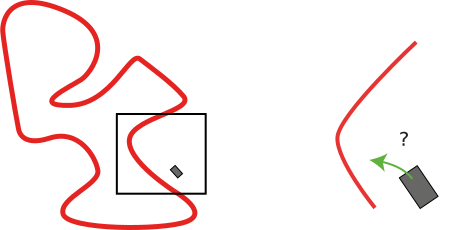
\includegraphics[width=1\textwidth]{image/schema_global.png}\\
\end{figure}


\section{Présentation du modèle : bicycle model}
\subsection{Présentation du bicycle model}
Pour modéliser une voiture, on utilise en général le modèle d'Ackermann. Cependant, nous voulons ici simplifier le model, pour cela une méthode très courante est d'utiliser le bicycle modèle.


\begin{figure}[h!]
    \centering
    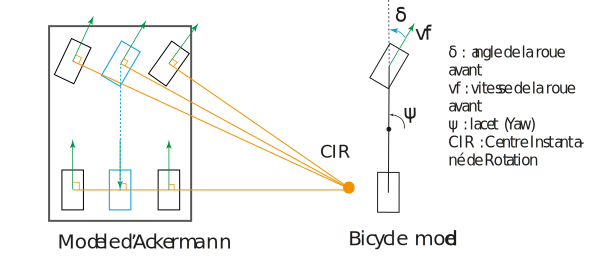
\includegraphics[width=0.9\textwidth]{image/Bicycle_model.png}\\
\end{figure}

\subsection{Cinématique}
Voici la cinématique d'un bicycle model, j'utilise les notations de la convention SAE (Society of Automotive Engineers)

\begin{figure}[h!]
    \centering
    \includegraphics[width=1\textwidth]{image/bicycle_Model_cinematic.png}\\
\end{figure}

En prenant $C =(x,y)$ et $w=\dot{\psi}$. On peut ainsi déterminer les 3 états $(x,y,\psi)$ de la voiture : 
\begin{equation*}
    \begin{cases}
        \dot{x} = v\cdot\cos(\psi + \beta) \\
        \dot{y} = v\cdot\sin(\psi + \beta) \\
        \dot{\psi} = \frac{v}{R} \\
    \end{cases}
\end{equation*}

Nous voyons ici que l'équation est déterminée avec $R$ qui est une inconnue.
Nous pouvons déterminer $\delta$ par rapport aux caractéristiques géométrique de la voiture.
\begin{equation*}
    \tan\delta = \frac{l_f+l_r}{R'} 
    \Leftrightarrow  R'= \frac{l_f+l_r}{\tan\delta}
\end{equation*}

\begin{equation*}
    \tan\beta = \frac{l_r}{R'}
    \Leftrightarrow \tan\beta = \frac{l_r}{l_r+l_f}\cdot\tan\delta
\end{equation*}    

\begin{equation*}
    \cos\beta = \frac{R'}{R} \Leftrightarrow \frac{1}{R} = \frac{\cos\beta}{R} = \frac{\cos\beta \cdot \tan\delta}{l_f+l_r}
\end{equation*}
On trouve ainsi l'équation qui régit la voiture : 
\begin{equation}
\boxed{
\text{Bicycle model temporel : }
     \left .
   \begin{dcases}
        \dot{x} = v\cdot\cos(\psi + \beta) \\
        \dot{y} = v\cdot\sin(\psi + \beta) \\
        \dot{\psi} = \frac{v}{l_r+l_f}\cdot\cos\beta\cdot\tan\delta \\
   \end{dcases}
   \right .
   avec \ \beta = \arctan(\frac{l_r}{l_r+l_f} \cdot \tan\delta) 
}
\end{equation}

Avec les simplifications suivantes :
\begin{equation*}
    \begin{array}{l}
        l_f=l_r\\
        L=l_r+l_f\\
        petit \ angle \rightarrow \beta \sim 0 , \ \tan(\delta) \sim \delta , \ \cos(\delta) \sim 1
    \end{array}
\end{equation*}

On a alors l'équation suivante :

\begin{equation}
\boxed{
    \text{Bicycle model temporel simplifié : }
    \begin{dcases}
        \dot{x} = v\cdot\cos(\psi) \\
        \dot{y} = v\cdot\sin(\psi) \\
        \dot{\psi} = \frac{v}{L}\cdot\delta \\
    \end{dcases}
}
\end{equation}

Le Path planning envoie un nouveau point objectif tous les \textbf{$T_e$ = 0.1 seconde}, il faut donc \textbf{discrétiser} les équations :

\begin{equation*}
     \begin{cases}
        X(k+1) = X(k) + T_e\cdot v\cdot\cos(\Psi(k)) \\
        Y(k+1) = Y(k) + T_e\cdot v\cdot\sin(\Psi(k)) \\
        \Psi(k+1) = \Psi(k) + \frac{T_e\cdot v}{L}\cdot\delta(k) \\
    \end{cases}
\end{equation*}

\begin{equation}
    \left .
    \Rightarrow
    \right . 
\boxed{
    \text{Bicycle model discret : }
    \begin{dcases}
        x(z) = \frac{T_e\cdot v\cdot\cos(\psi(z))}{1-z^-1} \\
        y(z) = \frac{T_e\cdot v\cdot\sin(\psi(z))}{1-z^-1} \\
        \psi(z) = \frac{T_e\cdot v}{L(1-z^1)}\cdot\delta(z) \\
    \end{dcases}
}
\end{equation}

On remarque que l'équation n'est pas linéaire à cause du $\cos$ et du $\sin$. J'ai donc cherché à les linéariser. Pour cela, j'ai utilisé un développement limité à l'ordre 1.
Ainsi, nous obtenons : 

\begin{equation}
    \left .
    \Rightarrow
    \right . 
\boxed{
    \text{Bicycle model discret linéarisé: }
    \begin{dcases}
        x(z) = \frac{T_e\cdot v}{1-z^-1} \\
        y(z) = \frac{T_e\cdot v\cdot\psi(z)}{1-z^-1} \\
        \psi(z) = \frac{T_e\cdot v}{L(1-z^1)}\cdot\delta(z) \\
    \end{dcases}
}
\end{equation}

J'ai les matrices du jacobien, ce n'est pas concluant pour l'instant :
\begin{equation*}
    A = 
    \left(\begin{array}{cccc}
        0 & 0 & -v\,\sin \left(\psi \left(t\right)\right) & 0\\
        0 & 0 & v\,\cos \left(\psi \left(t\right)\right) & 0\\
        0 & 0 & 0 & \frac{v}{L}\\
        0 & 0 & 0 & 0
        \end{array}\right) 
    \sim
    \left(\begin{array}{cccc}
        0 & 0 & -v\,\psi \left(t\right) & 0\\
        0 & 0 & v & 0\\
        0 & 0 & 0 & \frac{v}{L}\\
        0 & 0 & 0 & 0
        \end{array}\right) 
    \text{\ et \ } 
    B=\left(\begin{array}{c}
        0\\
        0\\
        \frac{v}{L}\\
        0
        \end{array}\right)
\end{equation*}    

Ainsi, grâce au jacobien on trouve que $\dot{X}$ : 
\begin{equation*}
    \dot{X} = \dot{X}_0 + \Delta \dot{X} =  
    \left(\begin{array}{cccc}
        x_0 & x_0 & x_0-\Delta x \cdot v\sin(\psi) & x_0\\
        y_0 & y_0 & y_0 + \Delta y \cdot v\cos(\psi) & y_0\\
        \psi_0 + \frac{\Delta \delta \cdot v}{L} & \psi_0 + \frac{\Delta \delta \cdot v}{L}  & \psi_0 + \frac{\Delta \delta \cdot v}{L}  & \psi_0 + \frac{\Delta \delta \cdot v}{L} + \frac{\Delta \psi\cdot v}{L} \\
        \delta_0 & \delta_0 & \delta_0 & \delta_0
        \end{array}\right) 
\end{equation*}  


\subsection{Dynamique}
Je ne vais pas traiter la dynamique du véhicule pour l’instant. Je vais d’abord essayer d’avoir un modèle simple qui fonctionne et que je comprends. J’étudierai le contrôle du véhicule avec un modèle dynamique plus tard.\\
\textcolor{red}{Traiter la dynamique du système.}


\section{Méthode de contrôle}
\subsection{Méthode géométrique : Pure Pursuite}
La méthode pure pursuite est la méthode humaine de piloter une voiture : on regarde, essaie en temps réel d'aller à un endroit situer devant nous. On définit cette distance grâce à $d$ la \emph{lookahead distance}.

\begin{figure}[h!]
    \centering
    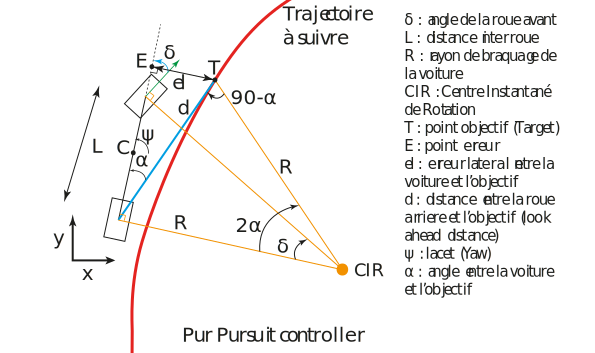
\includegraphics[width=1\textwidth]{image/Pure_pursuite.png}\\
\end{figure}

On remarque que 
\begin{equation*}
    \frac{d}{\sin(2\alpha)} = \frac{R}{\sin(\frac{\pi}{2}-\alpha)} 
    \iff
    \frac{d}{2\sin\alpha\cos\alpha} = \frac{R}{\cos\alpha}
    \iff
    \frac{1}{R} = \frac{2\sin\alpha}{d}
\end{equation*}

\begin{equation*}
    \tan\delta = \frac{L}{R} = \frac{2L\sin\alpha}{d}
\end{equation*}

\begin{equation*}
    \delta = \arctan(\frac{L}{R} = \frac{2L\sin\alpha}{d})
    \rightarrow petit \ angle \ 
    \delta = \frac{L}{R} = \frac{2L\sin\alpha}{d}
\end{equation*}

\begin{equation*}
    \sin\alpha = \frac{e_l}{d}
    \rightarrow petit \ angle \ 
    \alpha = \frac{e_l}{d}
\end{equation*}
\begin{equation*}
    \boxed{
    \text{Pure Pursuite : }
    \delta = \frac{2 L}{d^2}\cdot e_l
    }
\end{equation*}

On cherche la distance $e_l$ entre $E$ et $T$.\\
$T = (x_T,y_T)$\\
$E = (x_C+(\frac{L}{2}- d\cos\alpha)\sin(\psi), y_C+(d\cos\alpha-\frac{L}{2})\cos(\psi))$\\\\

En approximant que $\cos\alpha \sim 1$, on trouve :\\
$E = (x_C + (\frac{L}{2}- d)\sin(\psi), y_C + (d-\frac{L}{2})\cos(\psi))$\\\\

On peut déterminer la distance entre $E$ et $G$ : \\
\begin{equation*}
    d(E,T) = e_l  = \sqrt{[x_T-x_C+(\frac{L}{2}- d)\sin(\psi)]^2 + [y_T-y_C+(d-\frac{L}{2})\cos(\psi)]^2}
\end{equation*}
 

 
En discret, nous faisons la différence latérale en le nouvel objectif par rapport au point E de la voiture actuelle :
\begin{equation*}
\boxed{
\begin{array}{l}
    d(E(k-1), T(k)) = e_l(k)  \\= \sqrt{[x_T(k)-x_C(k-1)+(\frac{L}{2}- d)\sin(\psi(k-1))]^2 + [y_T(k)-y_C(k-1)+(d-\frac{L}{2})\cos(\psi(k-1))]^2}
\end{array}
}
\end{equation*}

On cherche à linéariser cette fonction : \\
Pour cela nous allons faire des développements limités d'ordre 1 sur $el$ en temporelle car plus simple :

\begin{equation*}
    el^2 = (x_g - x_c + (\frac{L}{2}-d)\sin(\psi))^2 + (y_g - y_c + (d-\frac{L}{2})\cos(\psi))^2
\end{equation*}

On veut faire un développement limité de $(1+X)^\alpha = 1 + \alpha x $. Il faut donc que les termes aux carrées soient sous la forme $(1+x)$. 
On cherche donc que $(x_g - x_c + (\frac{L}{2}-d)\sin(\psi))^2 = (1+X)^2 \iff X =x_g - x_c + (\frac{L}{2}-d)\sin(\psi)-1$. 
De même $Y = y_g - y_c + (d-\frac{L}{2})\cos(\psi) - 1$ et $E_l = e_l -1$.\\ Ainsi, nous avons l'équation suivante :

\begin{align*}
    & (E_l+1)^2=(X+1)^2+(Y+1)^2 \\
    & \iff 1+2(e_l-1)=1+2(x_g -x_c +(\frac{L}{2}-d)\sin(\psi)-1)+1+2(y_g-y_c+(d-\frac{L}{2})\cos(\psi)-1)\\
    & \iff e_l=x_g-x_c+y_g-y_c+(\frac{L}{2}-d)\cdot(\psi-1) - 0.5\\
\end{align*}

Ainsi, mettons cela en discret : 

\begin{align*}
    &e_l(k)=x_g(k)-x_c(k-1)+y_g(k)-y_c(k-1)+(\frac{L}{2}-d)\cdot(\psi(k-1)-1) - 0.5\\
    &\iff  \boxed{e_l(z)=x_g(z)-z^-1\cdot x_c(z) +y_g(z) - z^-1\cdot y_c(z) + z^-1\cdot(\frac{L}{2}-d)\cdot \psi(z) - (0.5 + \frac{L}{2}-d)}\\
\end{align*}

\subsection{Méthode black box : PID}
La méthode de la Black-box PID consiste à contrôler son véhicule sans avoir besoin de comprendre la cinématique, la dynamique, le comportement du véhicule avec un PID.

\begin{figure}[h!]
    \centering
    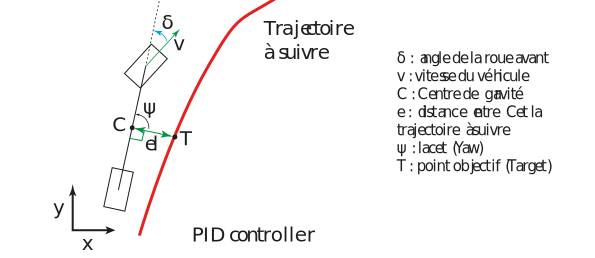
\includegraphics[width=1\textwidth]{image/PID.png}\\
\end{figure}

On cherche la distance entre $C$ et $G$:
\begin{equation*}
    d(T, C) = e_l= \sqrt{(x_T-x_C)^2+(y_T-y_C)^2}
\end{equation*}

En discret : 
\begin{equation*}
\boxed{
    d(T(k), C(k)) = e_l(k) = \sqrt{(x_T(k)-x_C(k-1))^2+(y_T(k)-y_C(k-1))^2}
}
\end{equation*}

\textcolor{red}{Mettre cette équation en \Large\textbf{z}}\\

\textbf{Il faut aussi transformer le correcteur PID en discret :} \\
Le PID en continu : 
\begin{equation*}
   \delta(t) = K_p \cdot e(t) + K_i \cdot \int_{0}^{t} e(t) \,dt + K_d \cdot \frac{de(t)}{dt}
\end{equation*}

Le PID en discret :
\begin{equation*}
    \delta(k) = K_p \cdot e(k) + K_i \cdot \sum_{i=0}^{k} e_i + K_d \cdot \frac{e(k)-e(k-1)}{Te}
\end{equation*}

Le PID en z : 
\begin{equation*}
    \delta(z) = K_p \cdot e(z) + K_i \cdot \frac{Te\cdot z}{z-1} + K_d \cdot \frac{z-1}{Te \cdot z}
\end{equation*}

\section{Schéma-bloc}
\subsection{Aperçu}
\subsubsection{Distance entre la voiture et la trajectoire – Problème de \underline{régulation}}
On peut voir le contrôle  de la trajectoire comme un problème de régulation.

\begin{figure}[h!]
    \centering
    \includegraphics[width=1\textwidth]{image/regulation.png}\\
\end{figure}

\pagebreak

\subsubsection{Distance entre la voiture et la trajectoire – Problème d’\underline{asservissement}}
On peut aussi voir le contrôle  de la trajectoire comme un problème d'asservissement.

\begin{figure}[h!]
    \centering
    \includegraphics[width=0.9\textwidth]{image/asservissement.png}\\
\end{figure}

On choisit de prendre ça comme un problème d'asservissement.

\subsection{Schéma-bloc : Pure Pursuite}

\subsubsection{Temporel}

\begin{figure}[h!]
    \centering
    \includegraphics[width=0.95\textwidth]{image/PP_temps.png}\\
\end{figure}

\subsubsection{Discret}

\begin{figure}[h!]
    \centering
    \includegraphics[width=0.95\textwidth]{image/PP_discret.png}\\
\end{figure}

\subsection{Schéma-bloc : PID}
\subsubsection{Temporel}

\begin{figure}[h!]
    \centering
    \includegraphics[width=0.95\textwidth]{image/PID_temps.png}\\
\end{figure}

\pagebreak

\subsubsection{Discret}

\begin{figure}[h]
    \centering
    \includegraphics[width=1\textwidth]{image/PID_discret.png}\\
\end{figure}

\section{Matlab}
\subsection{Simulation du Pure Pursuit sur Simulink}

\begin{figure}[h]
    \centering
    \includegraphics[width=1\textwidth]{image/PP_matlab_temps.png}\\
\end{figure}

\subsection{Simulation du PID sur Simulink}
\textcolor{red}{À faire en suivant la même méthode que le Pure Pursuit}

\pagebreak
\section{TO DO}
\begin{todolist}
    \item[\done] Discrétiser en z les équations de $e_l$ pour le Pure Pursuite et le PID en utlisant $e_l^2$ pour simplifier la racine
    \item[\done] Passer par le jacobien pour simplifier le $\psi$ et ainsi faire les petit angle dans $e_l$ du Pur Pursuite
    \item Faire la dynamique du bicycle model
    \item[\fail] Décomposer le modèle du système en $\frac{\psi}{\delta} \rightarrow \frac{(\dot{x},\dot{y})}{\psi}$ \textcolor{red}{$\Rightarrow (\cos\psi,\sin\psi) \Rightarrow$ non linéaire !}
    \item Lire et résumer en MarkDown sur Obsidian 
    \begin{todolist}
      \item[\done] AMZ Driverless: The Full Autonomous Racing System
      \item[\done] Automatic Steering Methods for Autonomous Automobile Path Tracking
      \item Implementation of path tracking algorithms and trajectory optimization based on the extended kalman filter
      \item Robotics, Vision and Control - Chap 4, 5, 6
    \end{todolist}
    \item[\done] Faire un encadrer dans le schéma de stratégie sur path tracking / planning et indiqué que c'est du discret 
    \item[\done] matlab symbolic pour vérifier linéarisation
    \item[\done] matlab symbolic pour jacobien
    \item Avec les formules linéarisées du bicycle model linéarisé
    \begin{todolist}
        \item Faire simulink avec les nouvelles formules linéarisés
        \item Faire matlab log avec les nouvelles formules linéarisés
        \item Faire schema-bloc
     \end{todolist}
    
\end{todolist}

\pagebreak
\end{document}
